\documentclass{article} %
\usepackage{times}
\usepackage{graphicx}
\usepackage{subfigure}
\usepackage{natbib}
\usepackage{algorithm}
\usepackage{algpseudocode}
%
\usepackage{hyperref}

%
%
\newcommand{\theHalgorithm}{\arabic{algorithm}}

%
%
%
%

%
%
%
\usepackage[accepted]{icml2016}
\usepackage{url}
\usepackage{amsfonts}
\usepackage{amsmath}
\usepackage{color}
\usepackage{afterpage}
\usepackage{xr}
%
\usepackage[T1]{fontenc}

\newcommand{\fix}{\marginpar{FIX}}
\newcommand{\new}{\marginpar{NEW}}
\newcommand{\note}[1]{\textcolor{red}{\textbf{[Note: #1]}}}
\newcommand{\todo}[1]{\textcolor{red}{\textbf{[TODO: #1]}}}

\renewcommand{\topfraction}{0.95}   %
\renewcommand{\textfraction}{0.05}  %

\newcommand{\hjm}{Jiamin He}

%
%

%

%
%

%
%
\icmltitlerunning{Asynchronous Methods for Deep Reinforcement Learning}

\begin{document}
\twocolumn[
\icmltitle{Replicating Deep Convolution Generative Adversarial \\
Network using existing code}

\icmlauthor{\hjm}{hejm37@mail2.sysu.edu.cn} \\


%
]

%

%

%
\begin{abstract}

In this paper, we replicated the result of Deep Convolution Generative Adversarial Network using an existing code. We trained the neural network on a two core CPU and compared the result during the training steps and other generative model. We also use a nearest neighbor classification algorithm to evaluate the result of the training.

%

%
%
%

\end{abstract}

\vspace{-0.2cm}
% \input{01_intro}
% \input{02_related}
% \input{03_background}
% \input{04_method}


%
\vspace{-0.1cm}
\section{Experiments}
\label{sec:experiments}

%

\subsection{MNIST Dataset}
The MNIST dataset is a dataset of handwritten digits which is widely used in training image processing machine learning algorithm. It contains 60,000 training images and 10,000 testing images which are always called training set and testing set. As a dataset for classification algorithm, the MNIST dataset is a well sovled dataset, and it is known as a beginning dataset for a lots of image processing algorithm. In this paper, we use the dataset to testify the convolution version of well known GAN, DCGAN. Another reason to choose this dataset is dued to the computation resources.

% Implementation Details
\subsection{Implementation Details}
\textbf{Training setup}
In the training, we used Adam optimizer with $\beta_1=0.5$, $\beta_2=0.999$, and a fixed learning rate of 0.0002 for both generator and discriminator. The networks are only trains for 20K steps due to the computing resources limit. In every $k$ step the generator updates $k-1$ times and the discriminator updates one time, here $k=2$. We train the network with a mini-batch size of 128 using stochastic gradient descent.

\noindent \textbf{Network Architecture}
The network structure of generator is in Figure~\ref{networkArc} while the structure of discriminator is roughly symmetrical with the one dimensional output unit rather than 100 dimensional. Notably, we use fractional-strided convolutions in generator and strided convolutions in discriminator. The activation in generator for all layers are ReLU except the output layer which uess Tanh. And activation in discriminator are all LeakyReLU.


% Compared Approaches/ Training time
\subsection{Compared Training Step}
To inspect the learning process of DCGAN, we sampled a few generated image during the training. And we could see the generated image is becoming more confounding with the real MNIST image (Figure~\ref{steps}).

\textbf{5k steps}
Figure~\ref{sample25} is 196 images sampled after 5k steps of training. We can see that most the images have had a basic shape of corresponding label.


\begin{figure}[ht]
\begin{center}

\includegraphics[width=\columnwidth]{figures/sample_0025}
\caption{\label{sample25} Images sample after 5k steps of training}
\end{center}
\vspace{-0.45cm}
\end{figure}

\textbf{10k steps}
The images sampled after 10k steps of training show that it is easier to identify the digits on the images. But the thickness of the digits vary widely among the images. There is a great amount of digits are only partly visible.

\begin{figure}[ht]
\begin{center}
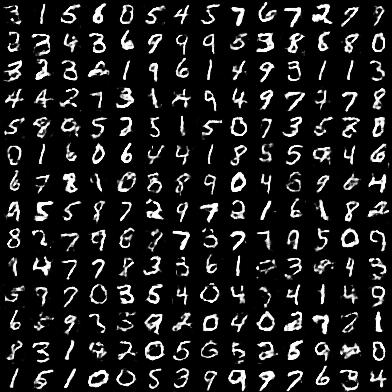
\includegraphics[width=\columnwidth]{figures/sample_0050}
\caption{\label{sample50} Images sample after 10k steps of training}
\end{center}
\vspace{-0.45cm}
\end{figure}

\newpage

\textbf{20k steps}
After 20k steps of training, the thickness problem improved a lot compared to 10k steps of training. We can see that most of the digits are plump enough as "human written digits". But still, there are some samples that are hard to recognize the digit on it.

\begin{figure}[ht]
\begin{center}

\includegraphics[width=\columnwidth]{figures/sample_0100}
\caption{\label{sample100} Images sample after 20k steps of training}
\end{center}
\vspace{-0.45cm}
\end{figure}


\begin{figure*}
\begin{center}
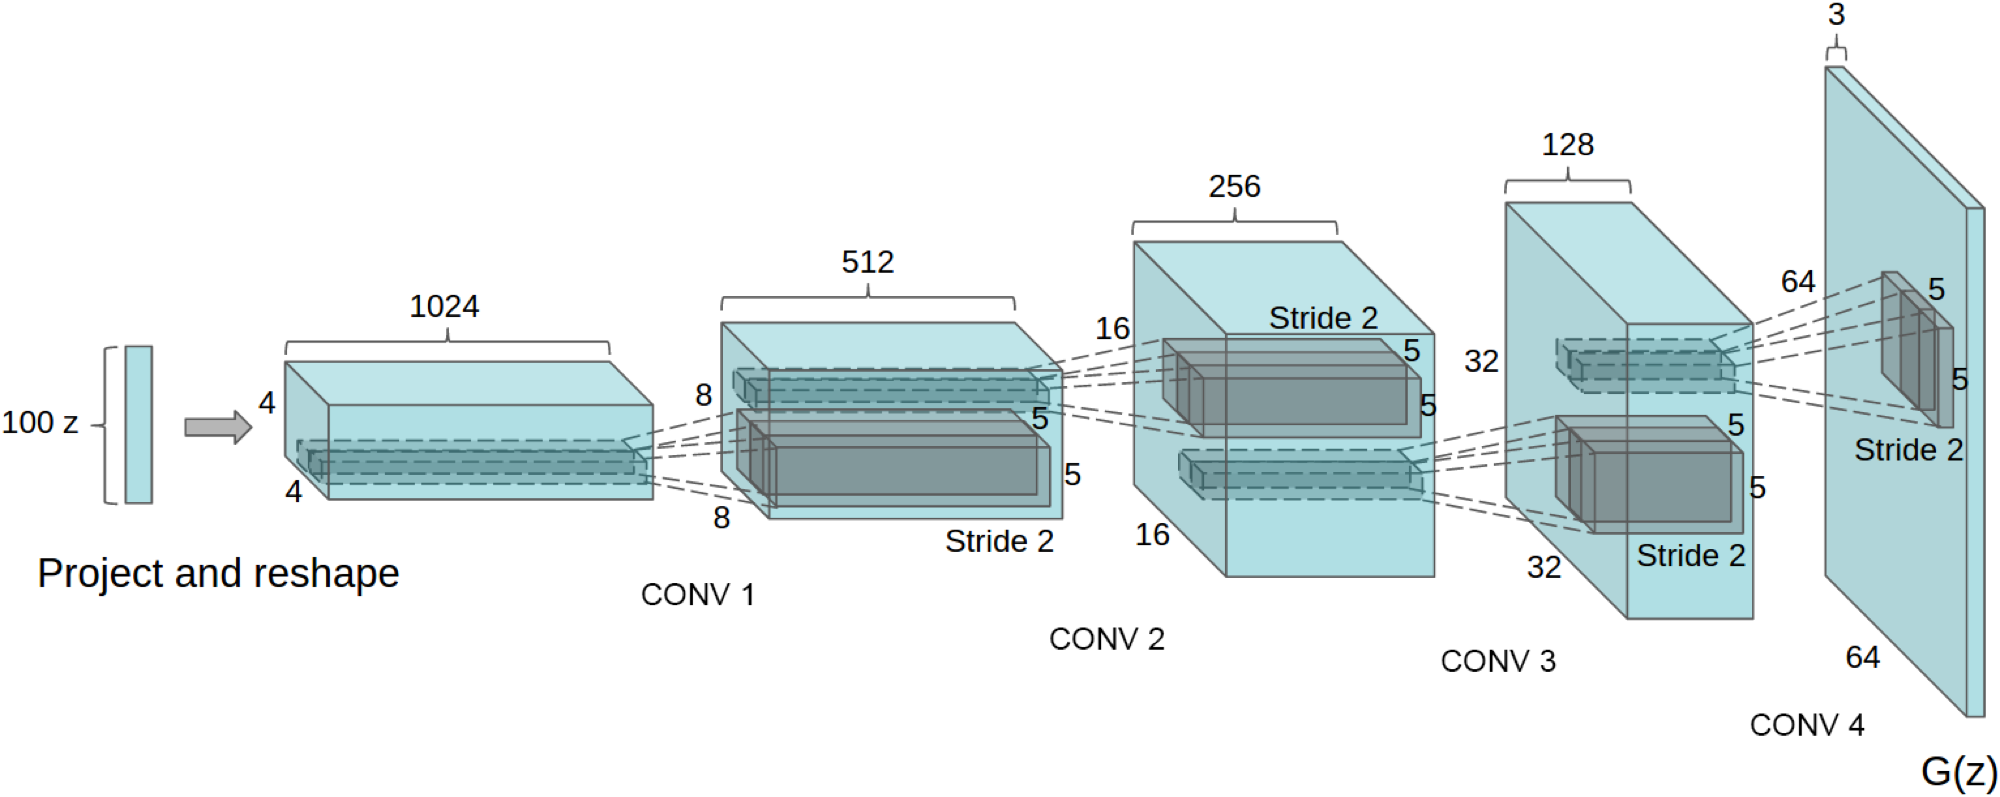
\includegraphics[width=\textwidth]{figures/networkArc}
\caption{\label{networkArc} A 100 dimensional uniform distribution $Z$ is projected to a small extent convolutional representation with many feature maps. A series of four fractionally-strided convolutions then convert this high level representation into a 64 $x$ 64 pixel image. Notably, no fully connected or pooling layers are used.}
\end{center}
\vspace{-0.45cm}
\end{figure*}



% Qualitative Results
\subsection{Qualitative Results}
% 对比MNIST原图,以及普通GAN网络
We compared our result with groundtruth MNIST, a baselines GAN and the origin paper \cite{DCGAN}. From Figure~\ref{compare} we can see that lacking of training, our result is still far behind the origin paper. The digit in origin paper are so well that it is hard to differ from the groundtruth MNIST. But we can also found that the digits generated by us are more plump and clear than that generated by GAN.

\begin{figure*}
\begin{center}
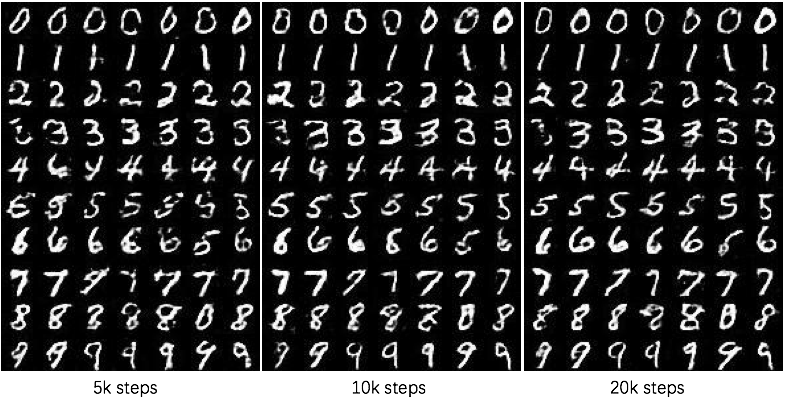
\includegraphics[width=\textwidth]{figures/steps}
\caption{\label{compare} Side-by-side illustration of (from left-to-right) generations after 5k steps, generations after 10k steps and generations after 20k steps.}
\end{center}
\vspace{-0.45cm}
\end{figure*}

\begin{figure*}
\begin{center}
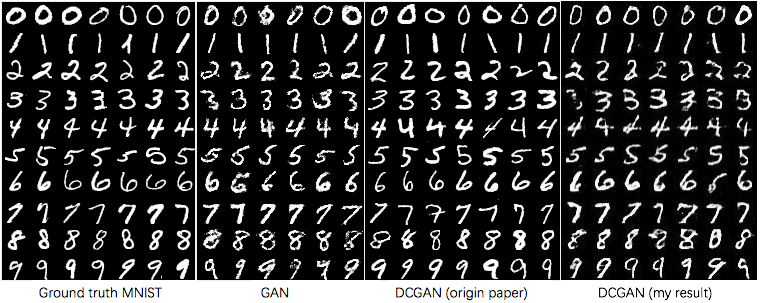
\includegraphics[width=\textwidth]{figures/compare}
\caption{\label{steps} Side-by-side illustration of (from left-to-right) the MNIST dataset, generations from a baselines GAN, generations from origin DCGAN \cite{DCGAN} paper and generations of our implementation.}
\end{center}
\vspace{-0.45cm}
\end{figure*}



% Quantitative Results
\subsection{Quantitative Results}
% 使用Nearest neighbor分类来对比DCGAN以及GAN、Real data的分类错误率
% Open-ai improved-gan, inception_score, https://github.com/openai/improved-gan/tree/master/inception_score
The mission of GAN is to train a network that the distribution of its output is simular to a given distribution. In this paper, we use the MNIST as the given distribution. We want the network to produce a distribution simular to the given data set. So same as the origin paper \cite{DCGAN}, we apply a standard classification metrics to evaluating the conditional distributions learned. We sampled 10192 images from our model (trained for 20k steps) and evaluated the models using k nearest neighbor classifier comparing real data to a set of generated conditional samples. We could see that only train the model for 20k steps is still not enough. 

\begin{table}[h]
\small
\begin{center}
\begin{tabular}{ | c | c | c | }
\hline
Method & Test Error (50K) & Test Error (10K) \\ \hline
Real Data & 3.1\% & -  \\
GAN & 6.28\% & -  \\
DCGAN (origin) & 2.98\% & -  \\ \hline
Real Data (ours) & - & 3.22\% \\
DCGAN (ours) & - & 5.19\% \\ \hline
\end{tabular}


\caption{\label{results} Nearest neighbor classification results 
%
%
}
\end{center}
\vspace{-0.45cm}
\end{table}

%
%
%
%
%
%
%

%
%
%
%
%
%
%
%
%
%
%


% \input{06_conclusion}

\subsubsection*{Acknowledgments and Anouncement}
We would like to thank Austin FitzGerald. This paper is creating by the author in a course in SYSU which aims to teach the students to read and write scientific paper. The knowledge and skill in the paper does not belong to the author, if anything used in this paper does not contain a proper reference, the author would be pleased to receive an notification email and get things correct.
\clearpage
\bibliographystyle{icml2016}
\bibliography{dcgan}

\clearpage

\renewcommand{\thealgorithm}{S\arabic{algorithm}}
\renewcommand{\thefigure}{S\arabic{figure}}
\renewcommand{\theequation}{S\arabic{equation}}
\renewcommand{\thetable}{S\arabic{table}}

\oddsidemargin .25in    %
\evensidemargin .25in
\marginparwidth 0.07 true in
\topmargin -0.5in
\addtolength{\headsep}{0.25in}
\textheight 8.5 true in       %
\textwidth 6.0 true in        %
\onecolumn
% \input{07_supplementary}

\end{document}
